Se realizará la geolocalización de tres universidades en las cuales me gustaría hacer una maestría, las universidades en cuestión son:
\begin{enumerate}
	\item Universitat Politècnica de València (Valencia, España)
	\item University of British Columbia (Vancouver, Canadá)
	\item Universidad de Friburgo (Friburgo de Brisgovia, Alemania)
\end{enumerate}

\section{Universidad Politècnica de València}
La URL de la universidad es \textit{https://www.upv.es/es/}
\subsection{Usando ping en la terminal de comandos}
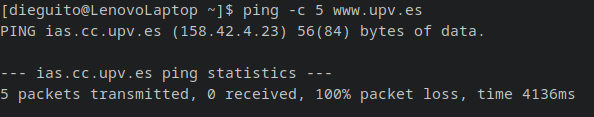
\includegraphics[scale=0.5]{ping-upv}\\
Al parecer la página no permite ser localizada mediante el comando ping.
\subsection{Dónde está el servidor que guarda la página}

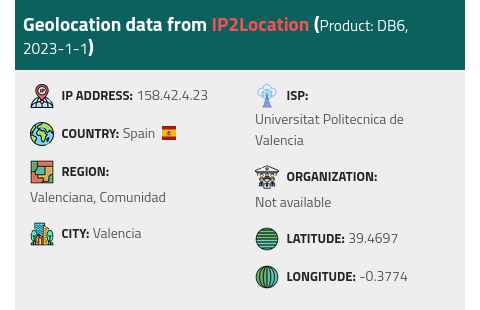
\includegraphics[scale=0.5]{iplocateupv}

La página iplocation.net muestra que la página está localizada en España, miremos si es exactamente en Valencia.

\subsection{Foto de Google Maps}

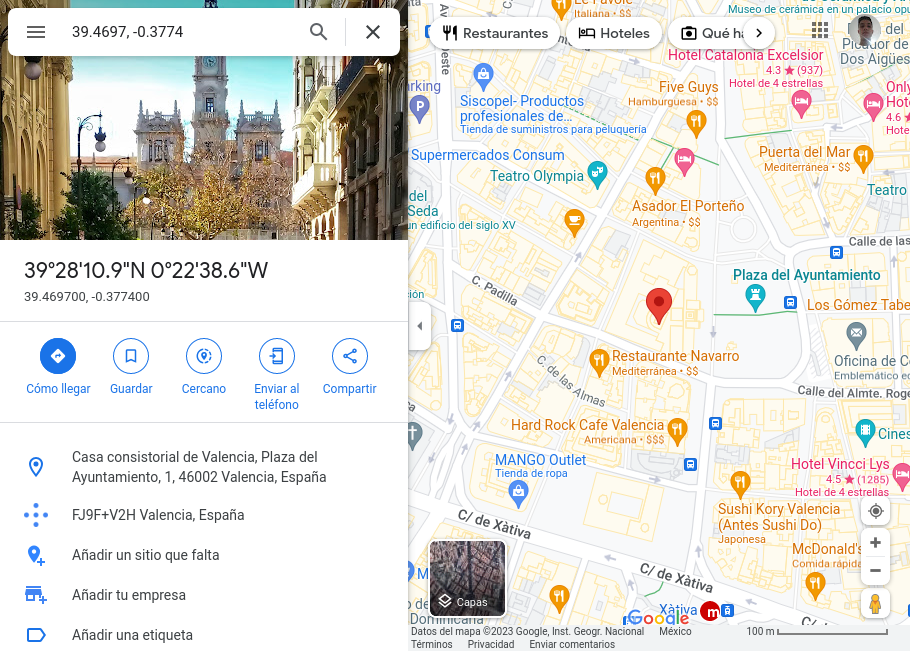
\includegraphics[scale=0.25]{maps-UPV.png}

Todo indica que sí se encuentra en Valencia, España.

\section{University of British Columbia}
La página es https://www.ubc.ca/
\subsection{Ping}
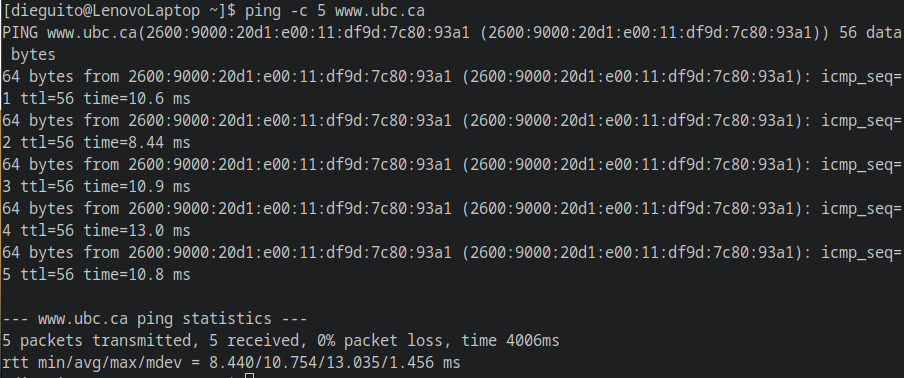
\includegraphics[scale=0.5]{ping-UBC}

La página respondió a los requests de ping, con un tiempo muy rápido para estar en Canadá, ¿verdad?

\subsection{¿Dónde está?}
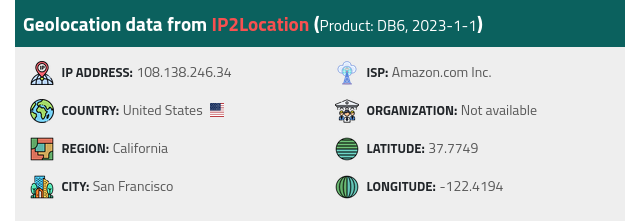
\includegraphics[scale=0.5]{ip-UBC}\\
Pues parece ser que está utilizando un proveedor de hosting.\\
\subsection{Verificando si está donde se dice}
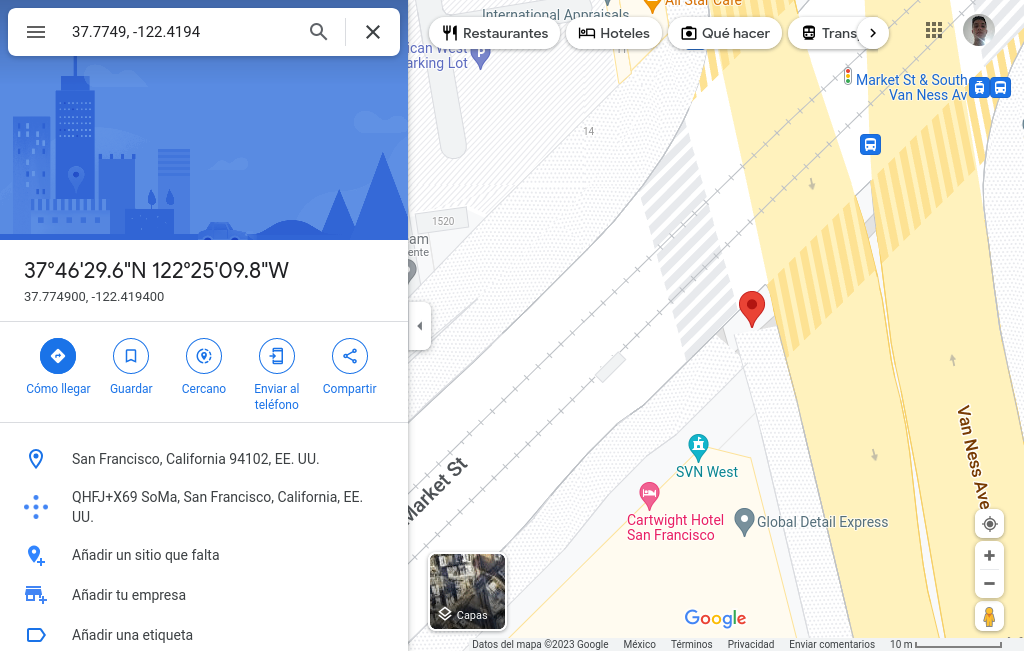
\includegraphics[scale=0.25]{maps-UBC}

Utiliza Amazon como su IAAS, conveniente.

\section{Universidad de Friburgo}
	\subsection{Ping}
	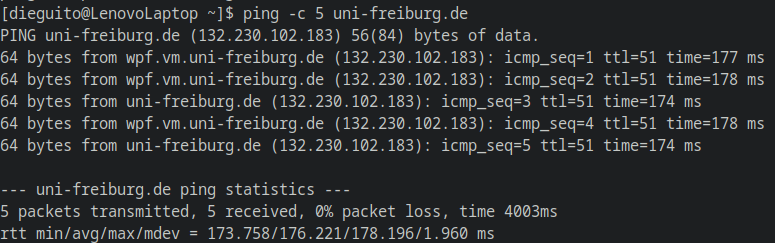
\includegraphics[scale=0.35]{ping-UF}\\
	Con un tiempo de respuesta lento, parece
	que está muy lejos.
	\subsection{Dónde está}
	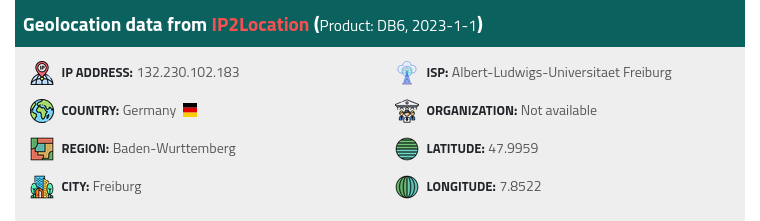
\includegraphics[scale=0.5]{ip-UF}\\
	Correcto, está lejos.
	\subsection{Foto de Maps}
	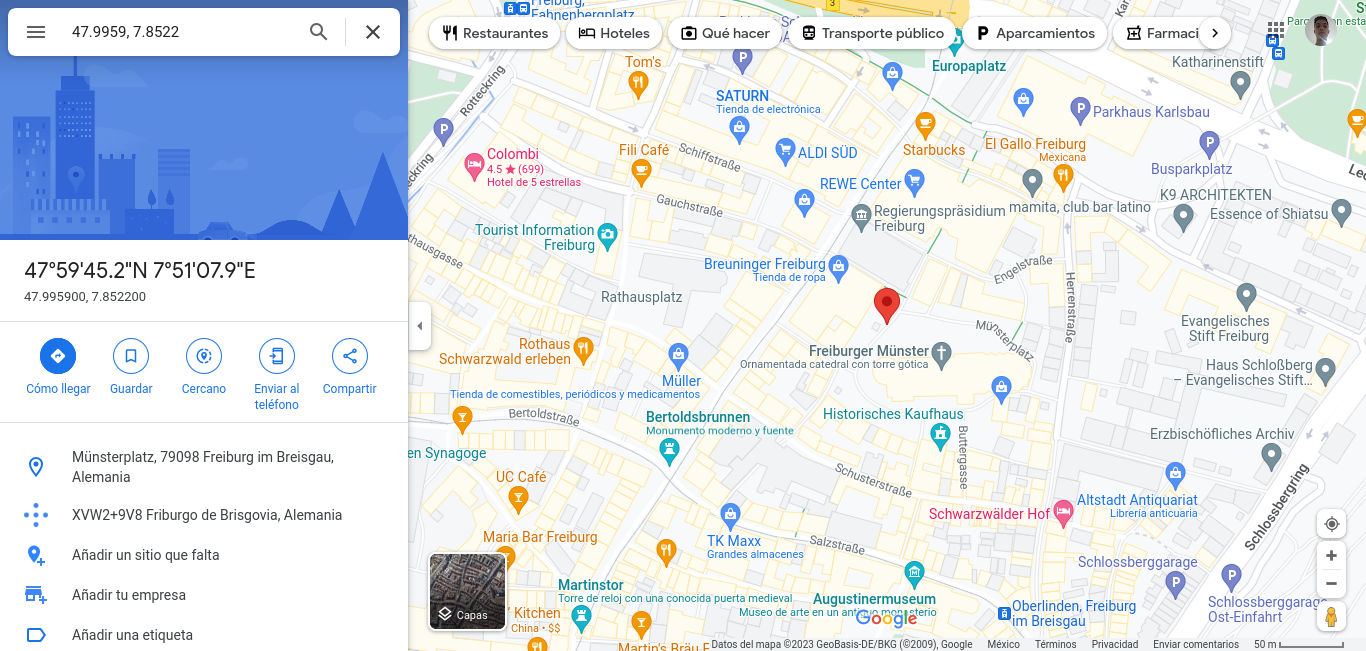
\includegraphics[scale=0.25]{maps-UF}	
	
\section{Una universidad más}
Como una de las universidades usa un servicio
de hosting, agregaremos una más para verificar
que esté en el lugar donde reside la misma;
la UNAM (Ciudad de México, México)
\subsection{Ping}
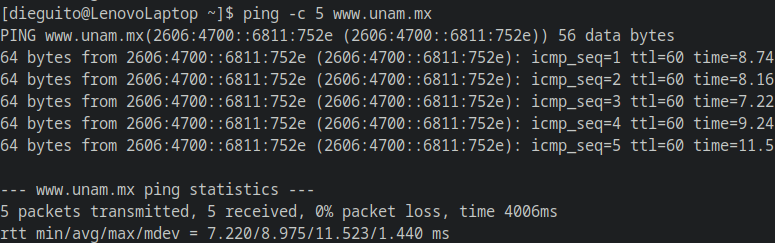
\includegraphics[scale=0.5]{ping-UNAM}\\
Todo bien hasta ahora, una respuesta rápida, pero no tanto como los servidores de Amazon en San Francisco.

\subsection{Localización}
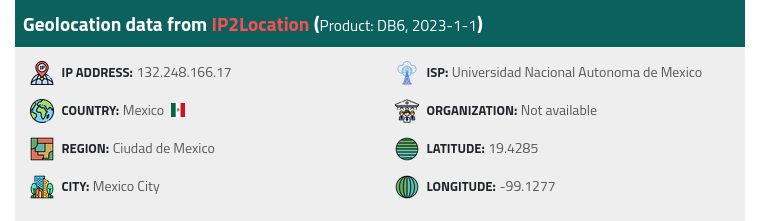
\includegraphics[scale=0.35]{ip-UNAM}\\
La página da que el servidor está en México.
\subsection{Google Maps}
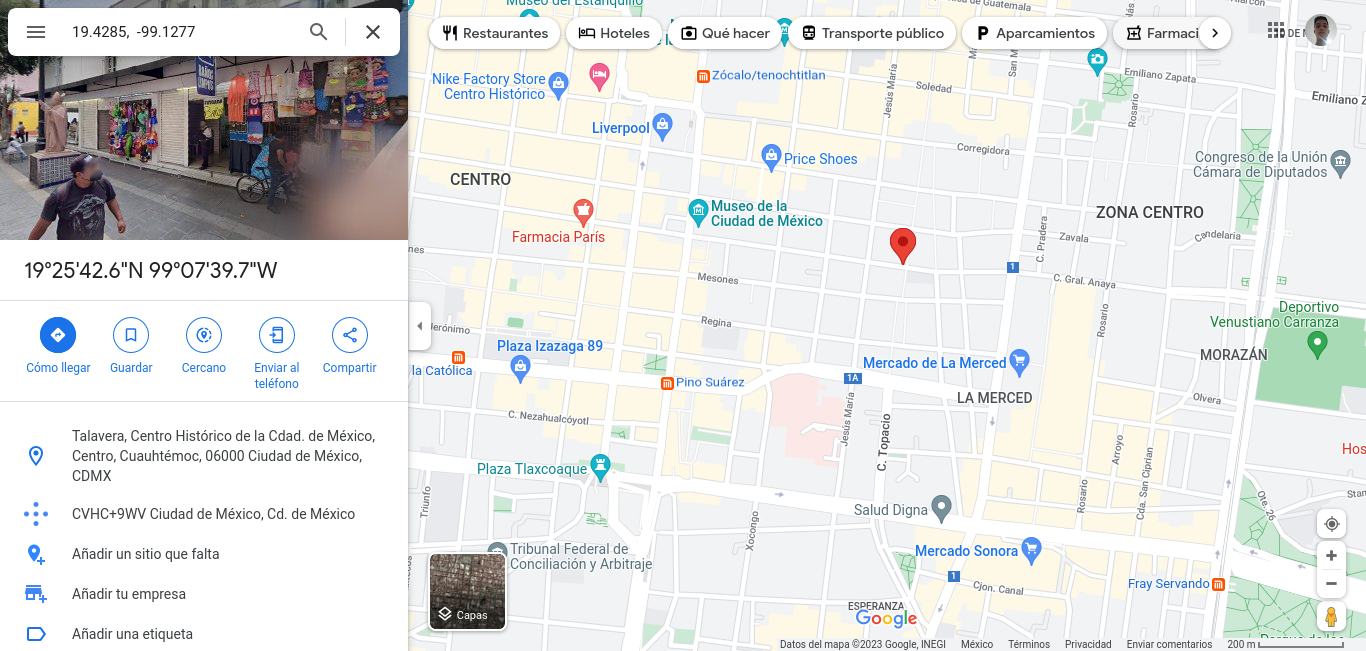
\includegraphics[scale=0.25]{maps-UNAM}\\
Pero al parecer no es nada cerca al campus,
o al menos eso parece.
	
	\section{Conclusión}
	Una de las tres universidades mencionadas (University of British Columbia) utilizó un 
	IAAS para su página web. Quizá le salía a
	costo rentar el servicio, a pesar que
	cuenta con un departamento de IT.
	No se culpa, es muy conveniente
	delegar y enfocarte en lo que te especialices;
	en este caso, la educación, mas no justifica
	el poder usar a tu staff académico para poder
	siquiera cotizar un salón con servidores para
	inversión. Tendrán sus razones muy válidas.
	
	